\subsubsection{Brief introduction to COCOMO II}
COCOMO (COnstructive COst MOdel) is a cost estimation algorithm allowing to estimate the time, effort and money needed to develop a project. It provides an empirical non-linear model based on two series of values:
\begin{itemize}
	\item\textbf{Scale Factors}, providing a gross estimate of the effort needed for the project.
	\item\textbf{Cost Drivers}, which can be \textit{Early Design} or \textit{Post-Architecture} and are applied to the effort as a multiplier.
\end{itemize}
COCOMO was originally published in 1981, based on a study of 63 projects of varying size and languages. COCOMO II, published in 2000, extends COCOMO by savoiding several underlying assumptions, such as waterfall development and stable requirements, and separating \textit{Early Design} from \textit{Post-Architecture} effort multipliers.

The general formula for calculating the needed Person-Months is $$ PM = 2.94 \cdot Size^E \cdot \prod_{i=1}^{n} EM_i $$ where $$ E = 0.91 + 0.01 \cdot \sum_{i=1}^{5}ScaleFactor_i $$ and size is expressed in Kilo Source Lines of Code, possibly derived from Function Points.

This estimate is made after planning the architecture, so we will use the \textit{Post-Architecture} model.

\subsubsection{Scale Factors}
On the tables are marked in grey the values we believe appropriate.
\paragraph*{Precedentedness: Low}
We have never built any similar application, although the structure of the application is not different from other projects that we have worked on. Between the three of us, we have experience of Server-Client architectures, Database Management, persistency in web applications, and an extensive knowledge of algorithms.

\paragraph*{Development Flexibility: High}
Management did not impose a choice of framework, architecture or any set of constraints except the product goals. We were therefore free to choose how to build our project.

\begin{figure}[h!]
	\centering
	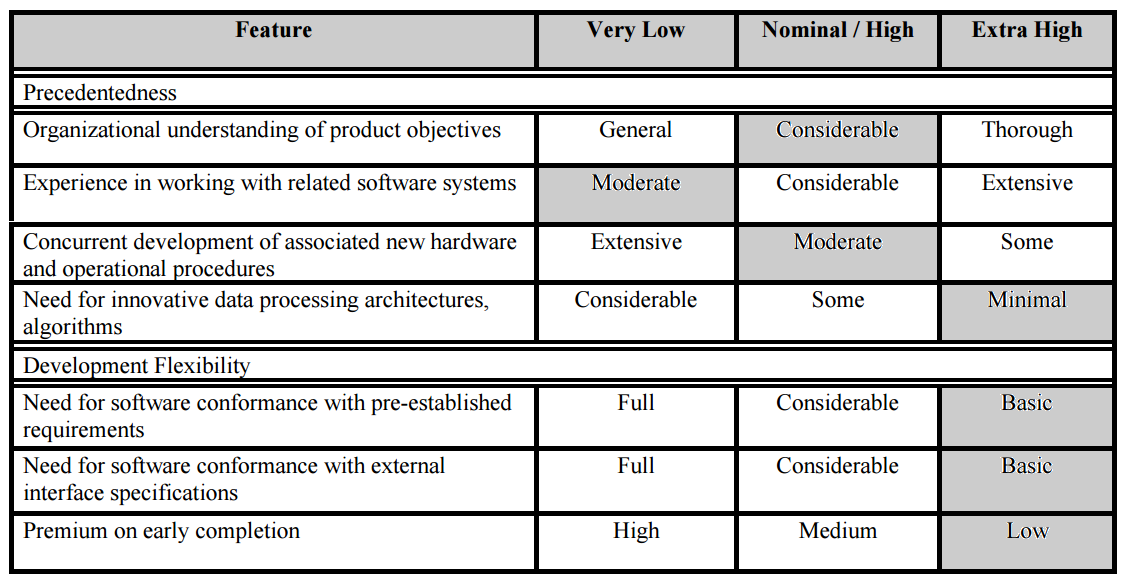
\includegraphics[width=\textwidth]{Images/PREC_FLEX}
	\caption{PREC and FLEX checklist}
\end{figure}

\paragraph*{Architecture/Risk Resolution: Low}
We were not provided with little information about risk management, budget and architecture, and had to work it out ourselves. We were allowed a high degree of freedom, and the company intervened into planning and periodic check, but we were provided little detail about the practical implementation of the preferred architectures and risk management.

\begin{figure}[h!]
	\centering
	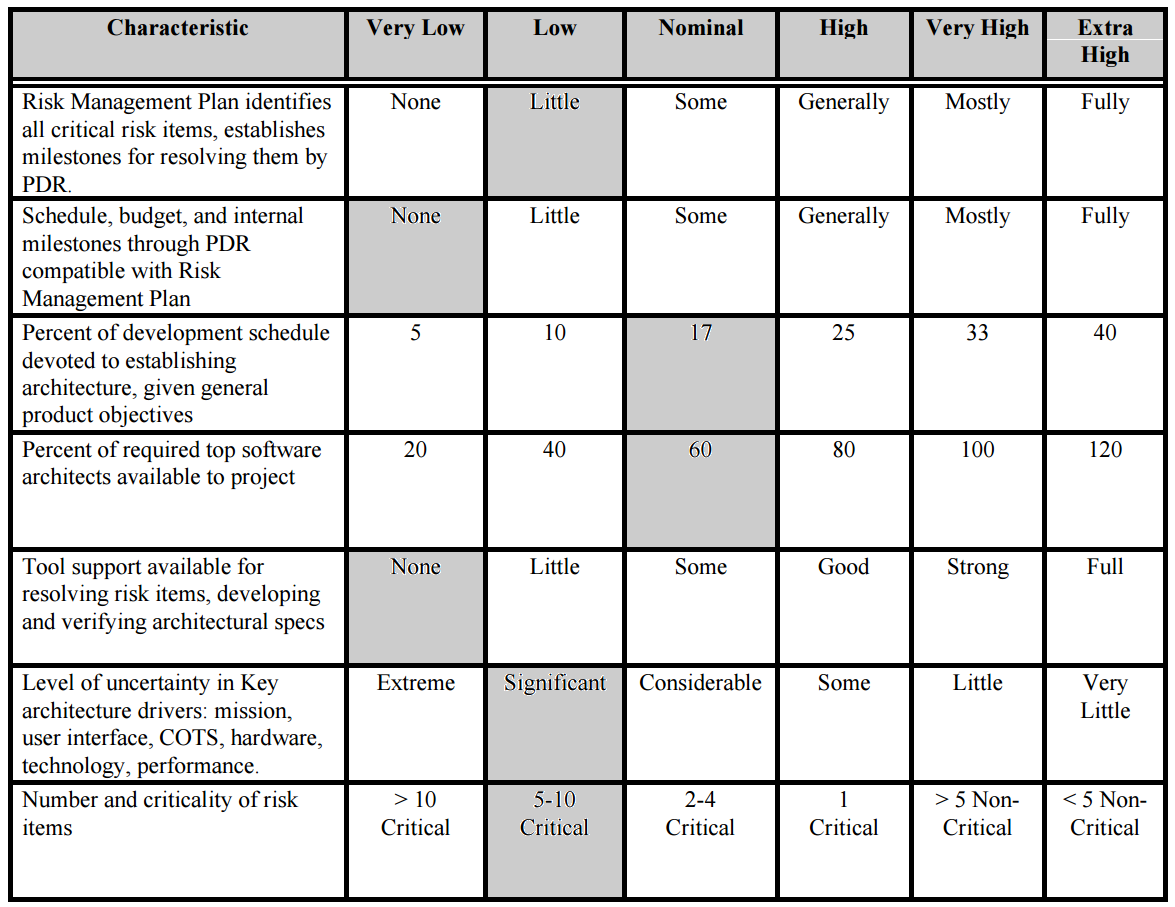
\includegraphics[width=\textwidth]{Images/RESL}
	\caption{RESL checklist}
\end{figure}

\paragraph*{Team Cohesion: High}
We had a couple of small misunderstandings early on, but managed to work them out and have been efficiently working together.

\begin{figure}[h!]
	\centering
	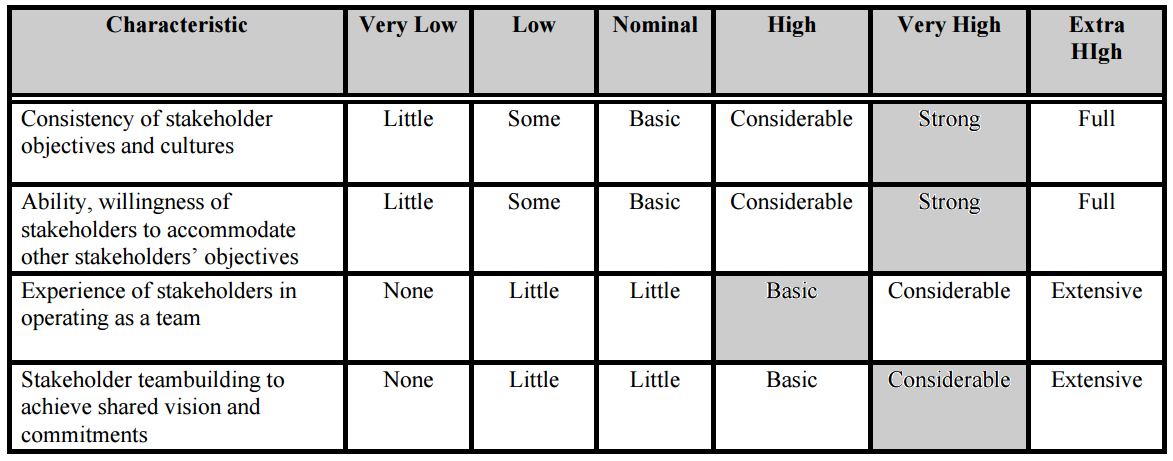
\includegraphics[width=\textwidth]{Images/TEAM}
	\caption{TEAM checklist}
\end{figure}

\paragraph*{Process Maturity: Nominal}
We believe the CMMI level to be around "Defined", accounting for our relative lack of experience but proactive attitude.

The process was managed, planned and executed by skilled people in accordance to a policy, planned together with the stakeholders, and produced controlled output. This satisfies the CMMI level 2.

In addition to that, the project was also defined at the organizational level, since our project would be the Company's main interface to the world. Additionally, we did all we could to proactively identify and address possible obstacles in the process. This satisfies CMMI level 3.

\subsubsection{Post-architecture Cost Drivers}
\paragraph*{Required Software Reliability: Nominal}
A service malfunction could cause inconvenience and non-trivial financial losses. This is because financial calculations are performed electronically, and a malfunction in the banking system could cause transaction losses. Additionally, Cars are locked and unlocked remotely, a lock service malfunction could lead to Cars being stolen.

\paragraph*{Data Base Size: Nominal}
The database size is standard for a medium-to-small-sized application. The database mainly stores data about Cars, Users, and Parking Areas. From an estimate of 12000 source lines of code, a nominal value is comprised between 120 KB and 1.2 MB, which is a reasonable estimate.

\paragraph*{Product Complexity: Nominal}
The product's complexity is par for the course for a medium-to-small-sized application. COCOMO provides a table for calculating it, which is reported and marked on the next page. The most complex part of the application is that relying on communication with the remote devices.

\begin{figure}[h!]
	\centering
	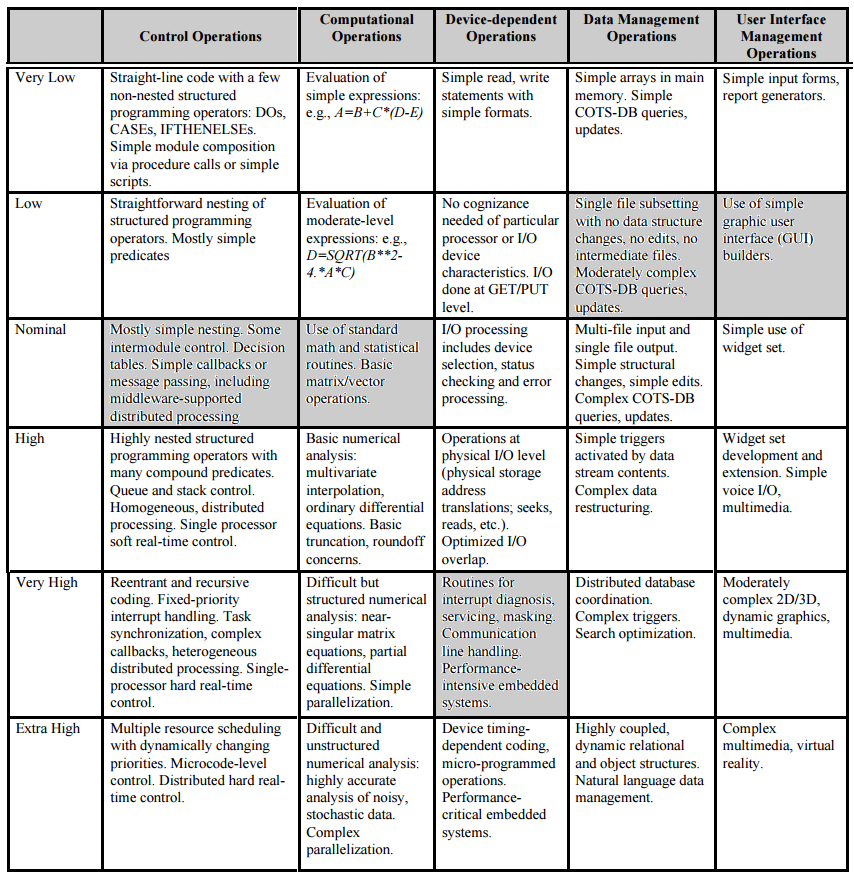
\includegraphics[width=\textwidth]{Images/CPLX}
	\caption{CPLX checklist}
\end{figure}


\paragraph*{Developed for Reusability: Nominal}
There was no specific reusability requirement, but we are working towards reusing components across the whole project whenever we do not need specialized components.

\paragraph*{Documentation Match to Lifecycle Needs: Nominal}
Adequately-sized documentation will be provided for the various stages of the project.

\paragraph*{Analyst Capability: Nominal}
We believe our skills to be around average, accounting for our relative lack of work experience. This project was designed during our course in Software Engineering 2, and we all passed Software Engineering I with good scores. We also cooperated extensively during the project.

\paragraph*{Programmer Capability: Nominal}
We believe our skills to be around average, accounting for our relative lack of work experience. We have all completed several courses of programming with good grades, showing efficiency and thoroughness,

\paragraph*{Personnel Continuity: Very High}
The three of us will keep working on the project from beginning to end.

\paragraph*{Application Experience: Low}
We have little experience in developing complete applications, but we have been working on parts of them in our previous courses. We believe 6 months' experience to be a good estimante.

\paragraph*{Platform Experience: Low}
We have little experience working with Spring, Tomcat and nginx. However, we have met several similar tools and platforms during our previous courses, so we believe 6 months' experience to be a reasonable estimate.

\paragraph*{Language and Toolset Exerience: Nominal}
We have a good understanding of Java, having used it across several courses. We are familiar with its built-in objects, main libraries, idioms, coding practices and with most Design Patterns. An estimate of 1 year's total experience is reasonable.

\paragraph*{Time Constraint: Very High}
The Central Service will consume the vast majority of the execution time, being up and running all the time (barring crashes) and tracking all the Cars In Use. So will the communication services, since rapid communication between the Cars, the User Application and the Central Service is essential for good software performance.

\paragraph*{Storage Constraint: Nominal}
No specific storage constraint was mentioned, and the amount of data created by the application is modest in size. We expect the application to use a storage percentage inferior to 50%.

\paragraph*{Platform Volatility: Low}
No major changes to any of the platforms (JavaEE, Spring, Tomcat, nginx) are expected to happen during the project, since they are all stable, mature platforms. Minor changesare expected, mostly in the form of software upgrades and patches.

\paragraph*{Use of Software Tools: High}
During development, several strong tools will be used to check on the lifecycle, such as mantaining a git repository. We will regularly update the repository with the latest source code, keeping the various design documents in the same place for easy access and accountability.

\paragraph*{Multisite Development: Extra High}
Most of the work will be done from home, coordinating through IRC and telephone. This way, there will be no time wasted in looking for a place to work together.

\paragraph*{Required Development Schedule: Nominal}
A rigid schedule was imposed on us for the first documents (RASD and DD), but we have more freedom for the project development. We will focus on concentrating our efforts in the early phases of development, in order to leave time for the unexpected.

\subsubsection{Effort Calculation}
By applying the algorithm (we used a free online tool, available at \\\texttt{http://csse.usc.edu/tools/COCOMOII.php}) based on our estimate of 236 FP, we obtained a result of 37.6 Person-Months, equivalent (considering a 160-hours work week) to 6016 Person-Hours.
\begin{figure}[h]
	\centering
	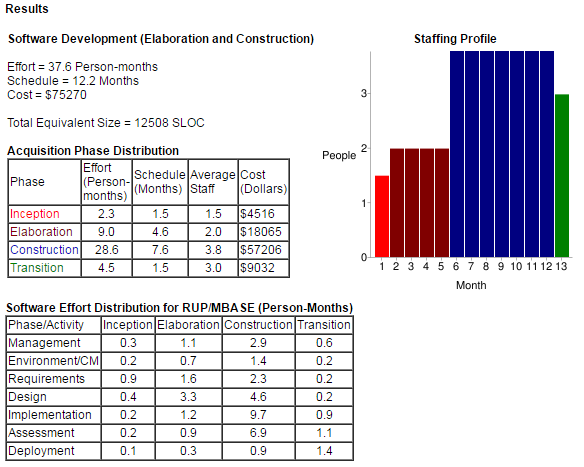
\includegraphics[width=\textwidth]{Images/COCOMO}
	\caption{COCOMO tool results}
\end{figure}

\subsubsection{Scheduling}
COCOMO provides an estimate of the project time frame through the formula $$ Duration = 3.67 \cdot Effort^{SE} $$ where $$ SE = 0.28 + 0.2 \cdot (E - 0.91) $$
resulting in an estimate of 12.2 months.

\subsubsection{Team Dimension}
The dimension of the team can be easily calculated as $\frac{Effort}{Duration}$, which, in our case, yields a result of 3.1. Since there are 3 of us, the duration will likely be extended.

This is also due to the fact that the amount of staff needed in the different phases of development is not constant: the construction phase would optimally require 4 people working. This can be avoided by hiring an additional developer, or extending the deadline. In the latter case, a realistic adjusted duration would be equivalent to 14.2 months, to reflect the increased time needed for the software construction.